% % % % % % % % % % % % % % % % % % % % % % % % % % % % % % % % % % % % % % % % % % % %
%                                                                                     %
% Short Sectioned Assignment LaTeX Template Version 1.0 (5/5/12)                      %
% This template has been downloaded from: http://www.LaTeXTemplates.com               %
%                                                                                     %
% Original author:  Frits Wenneker (http://www.howtotex.com)                          %
%                                                                                     %
% Modified by: Fco Javier Sueza Rodríguez (fcosueza@disroot.org)                      %
%                                                                                     %
% Changes:                                                                            %
%	    - Custom Chapters, Sections and Subsections (titlesec package)                %
%           - Document type scrbook (oneside)                                         %
%           - Use babel-lang-spanish package and marvosym                             %
%           - Use hyperref, enumitem, tcolorbox and glossaries packages               %
%           - Use Time New Roman (mathptmx), Helvetic and Courier fonts               %
%                                                                                     %
% License: CC BY-NC-SA 3.0 (http://creativecommons.org/licenses/by-nc-sa/3.0/)        %
%                                                                                     %
% % % % % % % % % % % % % % % % % % % % % % % % % % % % % % % % % % % % % % % % % % % %

%-----------------------------------------------%
%	              Packages                  %
%-----------------------------------------------%

\documentclass[paper=a4, fontsize=11pt, oneside]{scrbook}

% ---- Text Input/Output ----- %

\usepackage[T1]{fontenc}
\usepackage[utf8]{inputenc}
\usepackage{mathptmx}
\usepackage[scaled=.92]{helvet}
\usepackage{courier}
\usepackage[indent=12pt]{parskip}

\usepackage{geometry}
\geometry{verbose,tmargin=3cm,bmargin=3cm,lmargin=2.6cm,rmargin=2.6cm}

% ---- Language ----- %

\usepackage[spanish]{babel}
\usepackage{marvosym}

% ---- Another packages ---- %

\usepackage{amsmath,amsfonts,amsthm}
\usepackage{graphics,graphicx}
\usepackage{titlesec}
\usepackage{fancyhdr}
\usepackage{tcolorbox}
\usepackage{hyperref}
\usepackage{enumitem}
\usepackage[automake]{glossaries}

%--------------------------------------------------------------------%
%                      Customizing Document                          %
%--------------------------------------------------------------------%


% ----------- Custom Chapters, Sections and Subsections -------------- %

\titleformat{\chapter}[display]
			{\bfseries\Huge}
			{Tema \ \thechapter} {0.5ex}
			{\vspace{1ex}\centering}

\titleformat{\section}[hang]
			{\bfseries\Large}
			{\thesection}{0.5em}{}

\titleformat{\subsection}[hang]
			{\bfseries\large}
			{\thesubsection}{0.5em}{}

\titleformat{\subsubsection}[hang]
			{\bfseries\large}
			{\thesubsubsection}{0.5em}{}

\hypersetup{
    colorlinks=true,
    linkcolor=black,
    urlcolor=magenta
}

% ------------------- Custom heaaders and footers ------------------- %

\pagestyle{fancyplain}

\fancyhead[]{}
\fancyfoot[L]{}
\fancyfoot[C]{}
\fancyfoot[R]{\thepage}

\renewcommand{\headrulewidth}{0pt} % Remove header underlines
\renewcommand{\footrulewidth}{0pt} % Remove footer underlines

\setlength{\headheight}{13.6pt} % Customize the height of the header

% --------- Numbering equations, figures and tables ----------------- %

\numberwithin{equation}{section} % Number equations within sections
\numberwithin{figure}{section} % Number figures within sections
\numberwithin{table}{section} % Number tables within sections

% ------------------------ New Commands ----------------------------- %

\newcommand{\horrule}[1]{\rule{\linewidth}{#1}} % Create horizontal rule command


%----------------------------------------------------------------------------------------
%	TÍTULO Y DATOS DEL ALUMNO
%----------------------------------------------------------------------------------------

\title{
\vspace{10ex}
\normalfont \normalsize
\huge \textbf{Tarea 1: Implantación, Configuración y Administración de Servidores Web}
}
\author{Francisco Javier Sueza Rodríguez}
\date{\normalsize\today}

%----------------------------------------------------------------------------------------
%                                     DOCUMENTO
%----------------------------------------------------------------------------------------
\begin{document}


\maketitle

\thispagestyle{empty}

\vspace{68ex}

\begin{center}
    \begin{tabular}{l l}
        \textbf{Centro}: & IES Aguadulce \\
        \textbf{Ciclo Formativo}: & Desarrollo Aplicaciones Web (Distancia)\\
        \textbf{Asignatura}: & Despliegue de Aplicaciones Web\\
        \textbf{Tema}: & Tema 1 -  Implantación, Configuración y Administración de Servidores Web\\
    \end{tabular}
\end{center}

\newpage

\tableofcontents

\newpage
\section{Ejercicio 1: Arquitecturas Web}
\subsection{Enunciado}
Una plataforma o arquitectura web es el entorno empleado para diseñar, desarrollar y ejecutar un sitio web. Hay muchos modelos de plataformas y una de las piezas más importantes y determinantes a la hora de elegirla es el sistema operativo. Describe dos plataformas web, una basada en Linux y otra basada en Windows, indicando qué tecnologías utilizan para cada una de las capas, es decir, para cubrir aspectos como el servicio web (HTTP), el contenido dinámico, o el acceso a datos.

\subsection{Solución}

Una \textbf{plataforma web} es el conjunto de aplicaciones y tecnologías que nos permiten el desarrollo, despliegue y funcionamiento de una aplicación web. Aquí se van a comentar las dos más utilizadas en Linux y Windows, que son \textbf{LAMP} y \textbf{WISA}. Las cuales pasamos a analizar en la siguiente lista:

\begin{itemize}
    \item \textbf{L}inux, \textbf{A}pache, \textbf{M}ySQL y \textbf{P}HP (\textbf{LAMP})

    Esta es una de las plataformas de desarrollo web más empleadas en al actualidad, aunque podemos encontrar muchas variaciones. Por ejemplo, últimamente se esta empleando \textbf{PostgreSQL} como base de datos alternativa a MySQL, y el uso de \textbf{Python} en vez de \textbf{PHP} cada vez se esta extendiendo más, aunque aquí vamos a analizar la configuración original, que aún sigue usándose mucho.

    \begin{itemize}
        \item \textbf{Linux} (Sistema Operativo): como sistema operativo de esta plataforma se usa Linux, un sistema operativo basado en Unix y que desde sus inicios tiene una gran orientación al trabajo en red, permitiéndonos, prácticamente con la configuración por defecto, la puesta en marcha y administración de una gran variedad de servidores.

        \item \textbf{Apache} (Servicio Web): Apache es uno de los servidores web más usados en el mundo. Es desarrollado por una comunidad de voluntarios y supervisado por \textbf{The Apache Software Foundation}. En la plataforma LAMP, Apache será el encargado de proporcionar el \textbf{servicio web}, procesando las peticiones de los clientes y generando las respuestas adecuadas.

        \item \textbf{MySQL} (Acceso a Datos): esta base de datos, actualmente desarrollada por Oracle, también es una de las más ampliamente utilizadas. Utiliza el lenguaje \textbf{SQL} con algunas diferencias respecto a otras implementaciones. En la plataforma LAMP, MySQL será la encargada gestionar el \textbf{acceso a datos}, permitiendo la creación, modificación, eliminación y lectura de los datos necesarios para el funcionamiento de la aplicación web.

        \item \textbf{PHP} (Contenido Dinámico): este lenguaje de programación, que tiene ya unos cuantos años, es muy empleado en el desarrollo web desde hace mucho años. Y aunque hoy en día esta siendo sustituido por otros lenguajes como Java, Javascript, Ruby, Python, etc.., aún siguen siendo muy empleado, en parte debido a que Wordpress, uno de los gestores de contenido más usado en el mundo está desarrollado en este lenguaje. En esta plataforma, PHP se encargará de la \textbf{generación de contenido dinámico}, es decir, estará en la \textbf{capa de negocio} de nuestra plataforma.
    \end{itemize}

    \item \textbf{W}indows, \textbf{I}IS, \textbf{S}QL y \textbf{A}SP (\textbf{WISA})

    Esta plataforma de desarrollo web, también muy empleada en la actualidad, esta prácticamente desarrollada por \textbf{Microsoft}, usando en cada una de las capas diferentes aplicaciones desarrolladas por ellos. Es una plataforma más costosa que LAMP, ya que todo el software empleado es software propietario, pero también tiene muy buen soporte por parte de Microsoft.

    \begin{itemize}
        \item \textbf{Microsoft Windows} (Sistema Operativo): como sistema operativo esta plataforma usa Microsoft Windows, el sistema operativo más usado en PC actualmente, aunque en entornos de servidor Linux se usa más. Tiene diferentes versiones, algunas enfocadas más a los servidores que sus versiones de escritorio.

        \item \textbf{Internet Information Services} (Servidor Web): ISS es un servidor web y conjunto de aplicaciones y servicios incluidos en los sistemas Windows y que nos ayuda al despliegue de diferentes tipos de servicios, aunque en este caso, se usan para el despliegue y funcionamiento del \textbf{servidor web}, que se encargara de procesar las peticiones del cliente y generar las respuestas adecuadas.

        \item \textbf{SQL Server} (Acceso a Datos): SQL Server es un servidor de bases de datos desarrollado por Microsoft y uno de los más usados en la plataforma WISA. Al igual que MySQL en LAMP, proporcionará la infraestructura de base de datos para poder almacenar, leer, modificar y eliminar los datos que necesitará la aplicación para su funcionamiento.

        \item \textbf{Active Server Pages} (Contenido Dinámico): ASP es una tecnología que permite la generación de contenido web dinámico. Aunque no es un lenguaje de programación en si mismo, esta pensado para trabajar con otros lenguajes de programacón. Frecuentemente se asocia con la plataforma \textbf{.NET} de Microsoft y con el lenguaje de programación \textbf{C\#}, que en última instancia es el que nos permite realizar la programación de la plataforma.
    \end{itemize}
\end{itemize}

\section{Ejercicio 2: Clasificación de la Aplicaciones Web}
\subsection{Enunciado}
Enumera y explica brevemente cada una de las diferentes tecnologías asociadas a las aplicaciones web que se ejecutarán tanto del lado del servidor como del cliente, especificando lo que corresponde a cada uno de los casos.

\subsection{Solución}
En este ejercicio se van a enumerar y explicar la diferentes tecnologías web que se emplean tanto en el \textbf{lado el servidor} como en el \textbf{lado del cliente}, tal y como hemos visto en esta unidad, aunque también se añadirán algunas extras.

\begin{itemize}
    \item \textbf{Tecnologías del Lado del Servidor}
    \begin{itemize}
        \item \textbf{CGI (Common Gateway Interface)}: es uno de los estándares más antiguos que permiten que los clientes accedan a los programas que se ejecutan en el servidor, donde se generará el contenido dinámico. Actualmente esta cada vez más en desuso.

        \item \textbf{ASP (Active Server Pages)}: esta tecnología desarrollada por Microsoft se ejecuta en el lado del servidor y se encarga de generar el contenido dinámico. Actualmente se emplea \textbf{ASP.NET}, que es la evolución de ASP y que se integra con la plataforma de desarrollo \textbf{.NET}, que es un entorno de desarrollo que integra lenguajes, bibliotecas, herramientas, etc...

        \item \textbf{Java}: este lenguaje de programación también se ejecuta en el lado del servidor y permite, mediante diferentes tecnologías como \textbf{JSP}, \textbf{JSF} y \textbf{servlets}, el desarrollo de páginas web dinámicas encargándose de la generación de contenido. Actualmente se usa con diferentes bibliotecas y frameworks como \textbf{Spring Boot}, que aceleran enormemente los tiempos de desarrollo y crean aplicaciones web de mayor calidad.

        \item \textbf{PHP (Hypertext Preprocessor)}: es uno de los lenguajes interpretados del lado del servidor que más se ha usado en el desarrollo web. Es un lenguaje bastante potente que permite la interacción con diferentes bases de datos y la generación de contenido dinámico. Actualmente suele emplearse con algunos frameworks como \textbf{Laravel} que han introducidos mejoras sustanciales en el proceso de desarrollo agilizándolo y generando código de mayor calidad.

        \item \textbf{Javascript}: es el lenguaje de script por antonomasia del lado del cliente, pero con los años y el interés de poder desarrollar aplicaciones del lado del servidor con el se han desarrollado algunos frameworks, como \textbf{Node}, que nos permiten realizar aplicaciones en la parte del servidor aprovechando la enorme versatilidad que nos proporcionar Javascript. Recientemente, se esta empezando también a usar \textbf{Deno}, un fork de Node que incluye diferentes mejoras, aunque aún no esta tan extendido como el primero.

        \item \textbf{Python}: este lenguaje interpretado se esta empleando cada vez más en el desarrollo web de la parte del servidor. Es un lenguaje muy versátil y que genera código muy elegante y sencillo. Además, posee algunos frameworks especializados en el desarrollo web, siendo el más conocido \textbf{Django}, un framework orientado al desarrollo rápido de aplicaciones web.

        \item \textbf{Ruby}: este lenguaje de programación interpretado y orientado a objetos, surgió en 1995 y esta basado en lenguajes como Python, Perl o Smalltalk. Es un lenguaje que genera código muy limpio y elegante y que actualmente ofrece uno de los frameworks de desarrollo web más potentes, como es \textbf{Ruby On Rails}.
    \end{itemize}

    \item \textbf{Tecnologías del Lado del Cliente}:
    \begin{itemize}
        \item \textbf{HTML (HyperText Markup Language)}: HTMl es un lenguaje de marcado  basado en SGML y que actualmente es el estándar para la maquetación de páginas web, encontrándose en su versión HTML 5.

        \item \textbf{CSS (Cascading Style Sheet)}: es un lenguaje de diseño gráfico que permite definir la presentación de un documento estructurado en un lenguaje de marcado, por norma general HTML, y que hace posible la separación entre la presentación y la estructura de un página web. Actualmente suele emplearse con algunos preprocesadores como pueden se \textbf{SASS} o \textbf{SCSS}, que añaden funcionalidades al lenguaje.

        \item \textbf{Java}: aunque también podemos encontrarnos con Java en el lado del cliente, cada vez se suele usar menos, aunque su presencia en los primeros años de la web era enorme, ya que permite crear pequeñas aplicaciones, conocidas como \textbf{applets}, que se pueden insertar en la páginas web.

        \item \textbf{JavaScript}: el lenguaje más empleado en el entorno del cliente. Es un lenguaje interpretado que permite añadir interactividad a la página web sin necesidad de realizar peticiones al servidor. Actualmente todos los navegadores web lo soportan, aunque cada navegador implementa un motor de javascript diferentes, siendo los más comunes \textbf{Spidermonkey} o \textbf{V8}.

        \item \textbf{TypeScript}: este lenguaje, desarrollado por Microsoft, es una versión de JavaScript a la que se le han añadido algunas funcionalidades de las que carece JavaScript, como el \textbf{tipaado estático}, las \textbf{interfaces}, etc. Actualmente va ganando terreno, ya que proporciona todas las ventajas de JavaScript mejorando algunos de sus puntos flacos.

        \item \textbf{Librerías y FrameWorks}: aunque no es un tecnología concreta, cabe destacar que hoy en día la mayor parte del desarrollo de páginas web en el lado del cliente se lleva a cabo usando alguno de los diferentes framework y librerias para el front-end que podemos encontrar. La gran mayoría usa Javascript (o TypeScript) como base, siendo los más empleados \textbf{React.js}, \textbf{Vue.js} o \textbf{Angular}. Cada uno ofrece diferentes características, permitiendo más o menos libertad a la hora de desarrollar la web, aunque todos tienen algo en común, y es que aceleran enormemente los tiempos de desarrollo, y por lo tanto, los costes.
    \end{itemize}
\end{itemize}

\section{Ejercicio 3: Instalando Nuestro Servidor Web}
\subsection{Enunciado}
Dispones de una máquina (o máquina virtual) que cuenta con el sistema operativo Ubuntu 20/22 recientemente actualizado, con el entorno de red configurado y conexión a Internet. Además, estás trabajando con la cuenta del usuario root. Indica cada uno de los pasos, y comandos implicados en ellos, para conseguir hacer lo siguiente:

\begin{itemize}
    \item Instalar el servidor web Apache desde terminal de comandos.
    \item Arrancar, reiniciar, comprobar el estado y parar el servidor web Apache.
    \item Comprobar que está funcionando el servidor Apache desde un navegador web.
    \item Cambiar el puerto por el cual está escuchando Apache pasándolo al puerto 8088 y comprueba de nuevo desde tu navegador que está funcionando.
    \item Cambiar la página web por defecto para que aparezcan tus apellidos mas un pantallazo de tu inicio del curso.
\end{itemize}

\subsection{Solución}
En este ejercicio se va a realizar la instalación de \textbf{Apache 2} como servidor web en un sistema \textbf{Linux Ubuntu 22}. En mi caso, uso \textbf{Kubuntu 22.04 }como sistema operativo de escritorio, por lo que la instalación se realizará en este sin necesidad de máquina virtual, ya que solo difiere de Ubuntu en el gestor de ventanas por defecto, que es KDE en vez de Gnome.

Además de la instalación, se realizarán algunas tareas básicas de administración sobre el servidor instalado. En la siguiente lista, podemos ver todos los pasos y comandos empleados:

\begin{itemize}
    \item \textbf{Instalación de Apache}: en este caso, Apache2 ya esta instalado, ya que la instalación se realizó para la asignatura Desarrollo Web en el Entorno del Servidor. Para su instalación se utilizó el comando \textbf{APT}, en concreto \textbf{\textit{sudo apt-get install apache2}}, así que si ejecutamos dicho comando, no va a tener efecto. También están instalados todos los paquetes necesarios, por lo que se mostrará la salida del comando \textbf{apt list}, en su lugar, donde se muestra la correcta instalación de los paquetes, como vemos en la siguiente captura:

    \begin{figure}[H]
        \centering
        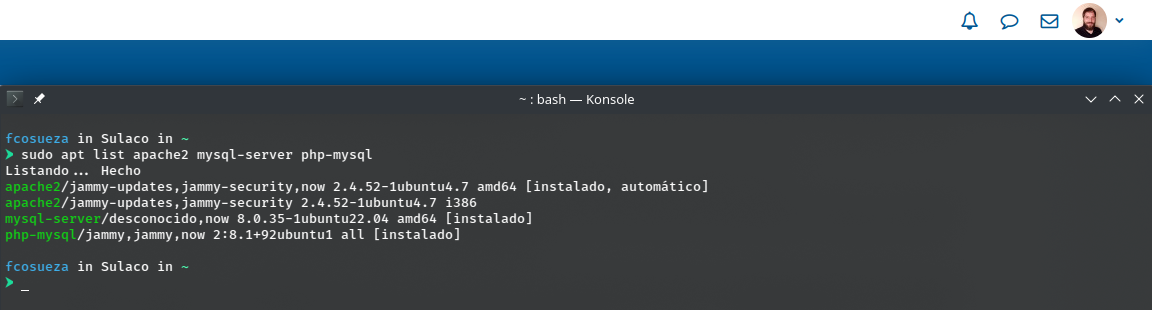
\includegraphics[scale=0.50]{apache-install.png}
    \end{figure}

    \item \textbf{Arranque, Parado y Estado de Apache}: para realizar estas labores de administración de ha usado el comando \textbf{\textit{service}} de Kubuntu, en concreto, los comandos empleados han sido, por orden: \textbf{\textit{sudo service apache2 start}}, \textbf{\textit{sudo service apache2 restart}}, \textbf{\textit{sudo service apache2 status}} y \textbf{\textit{sudo service apache2 stop}}, como podemos ver en la siguiente captura de la terminal.

    \begin{figure}[H]
        \centering
        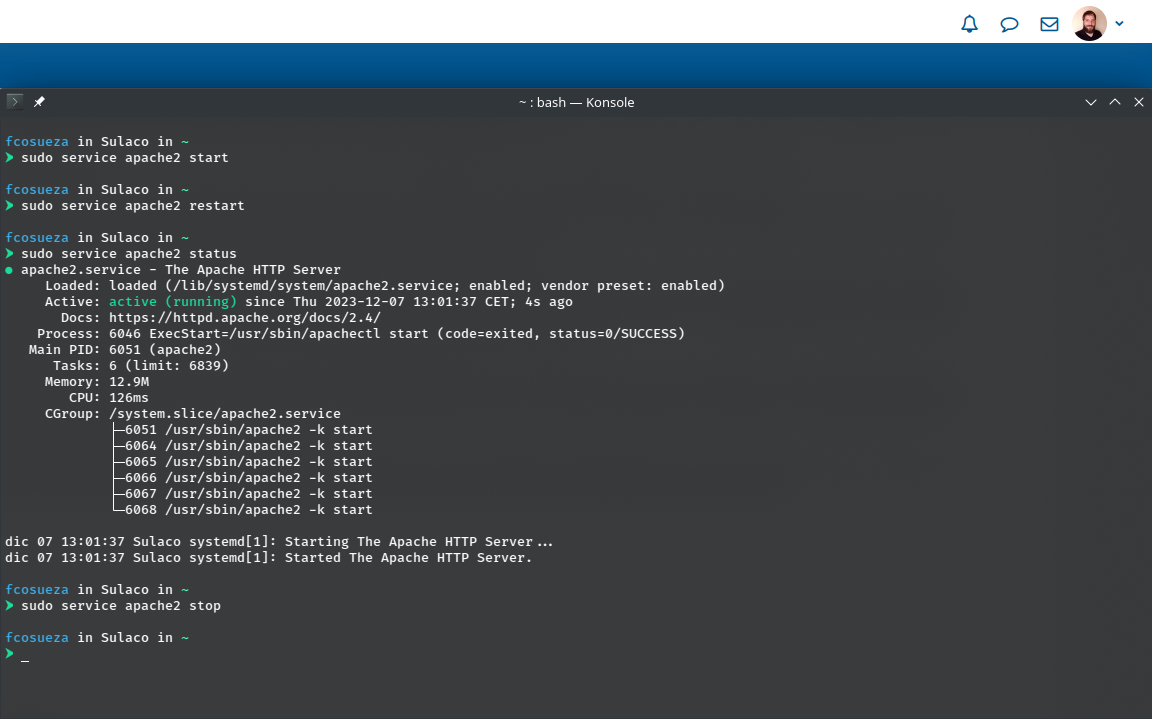
\includegraphics[scale=0.50]{apache-service.png}
    \end{figure}

    \item \textbf{Comprobar Instalación}: una vez realizada la instalación y probados algunos comandos básicos, vamos a comprobar que el servidor funciona correctamente, conectándonos a nuestro localhost desde el navegador, que como podemos ver en la siguiente captura, muestra la página por defecto de Apache2.

    \begin{figure}[H]
      \centering
     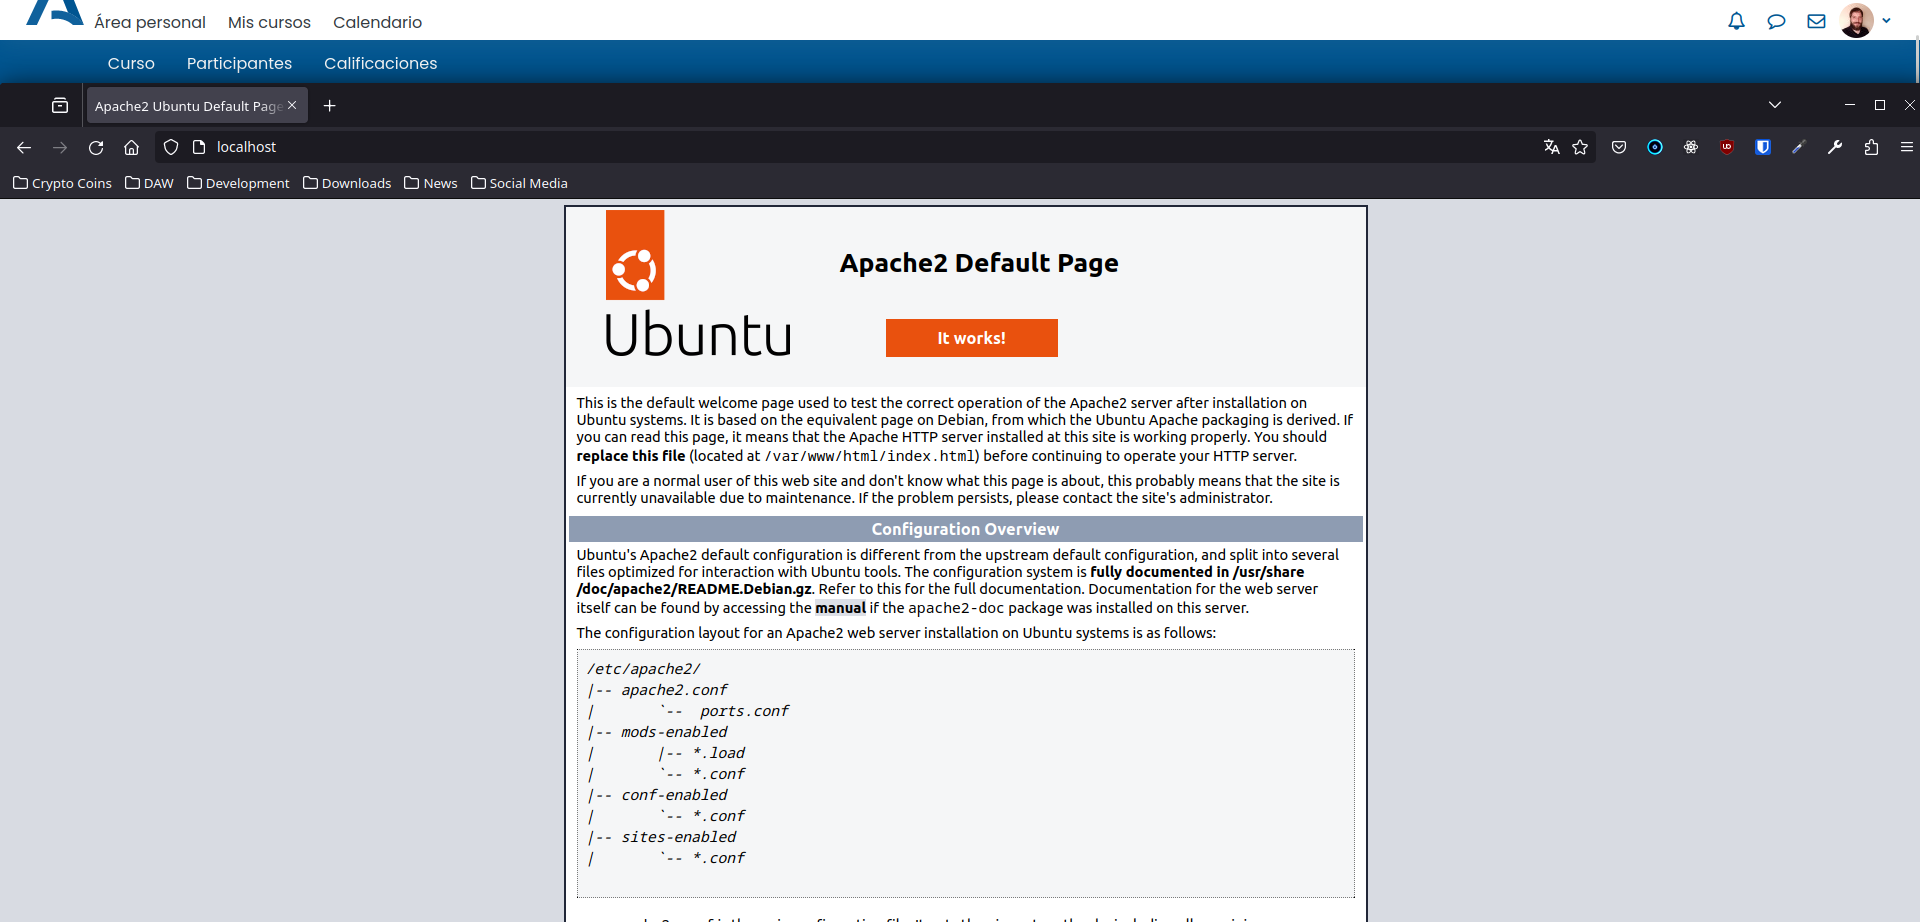
\includegraphics[scale=0.30]{apache-home.png}
    \end{figure}

    \item \textbf{Cambiar Puerto por Defecto}: para cambiar el puerto por defecto se ha consultado el archivo \textbf{/etc/apache2/apache2.conf}. En este fichero, se nos indica, mediante la directiva \textbf{Include ports.conf}, y su comentario asociado, que es en ese fichero donde debemos modificar los puertos en los que estará escuchando el servidor.

     Se ha editado ese fichero, cambiando la directiva \textbf{Listen 80} por \textbf{Listen 8088}. Tras reiniciar el servidor hemos comprobado su correcto funcionamiento conectando desde un navegador al localhost, pero cambiando el puerto de conexión 8080, como se puede ver en al siguiente captura.

     \begin{figure}[H]
         \centering
         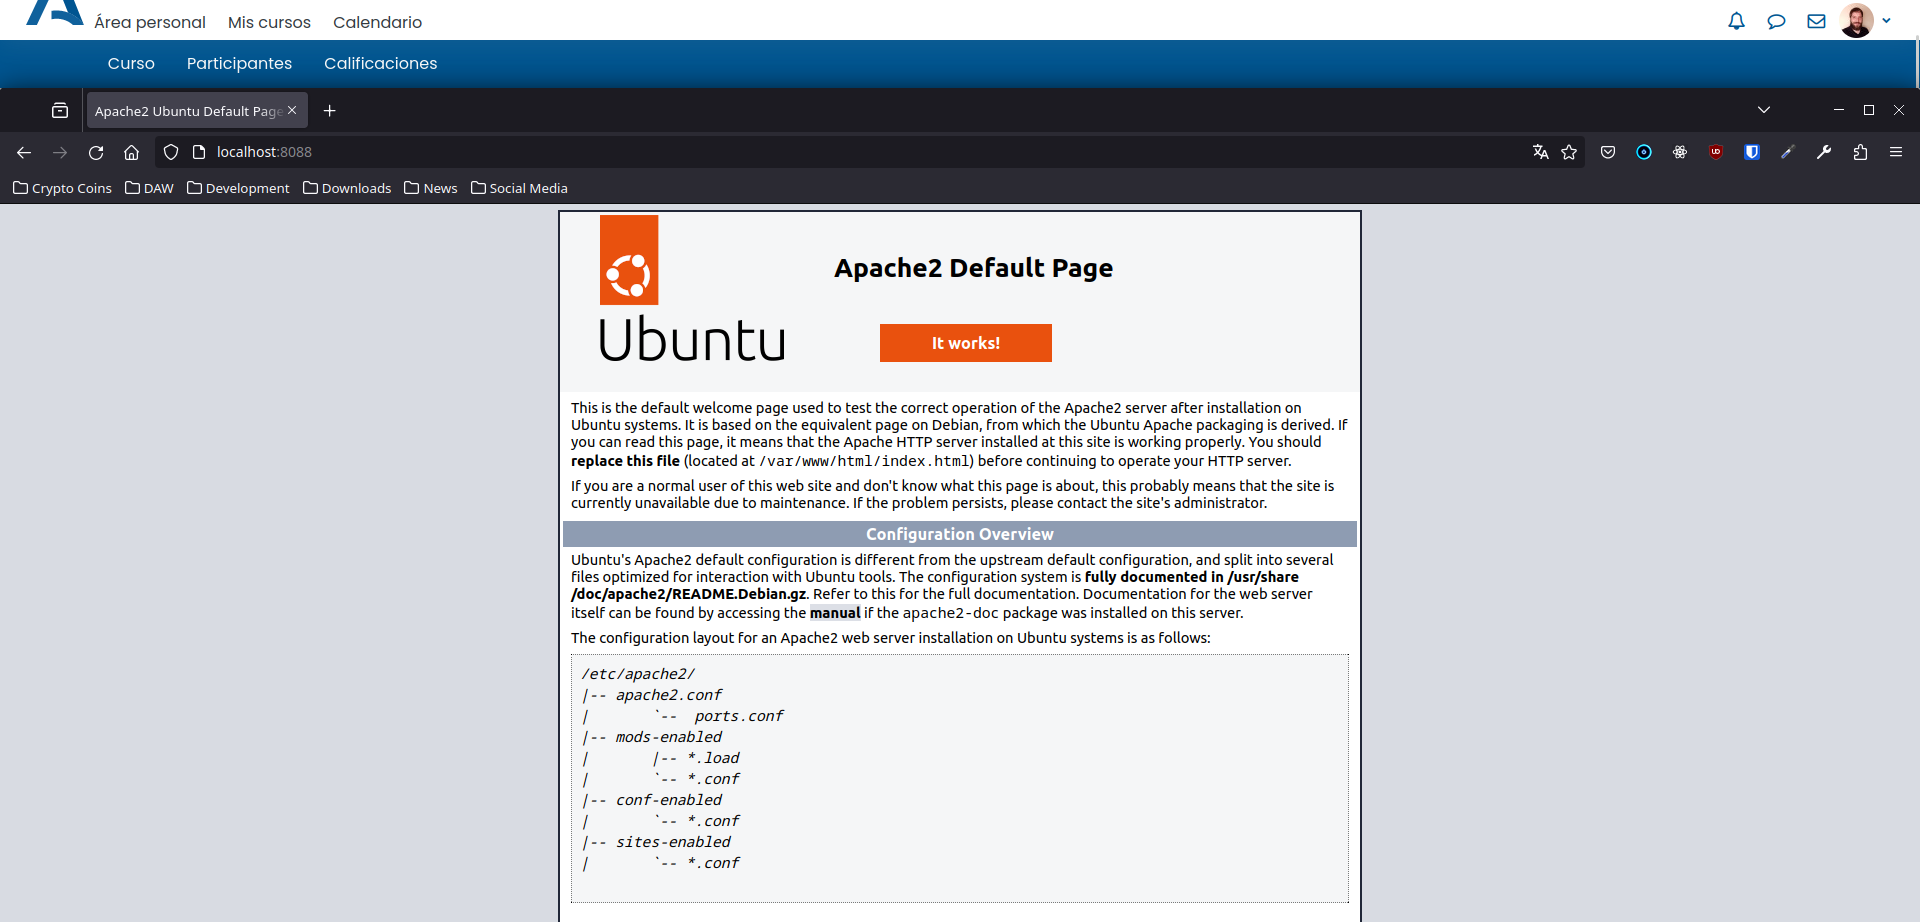
\includegraphics[scale=0.30]{apache-port.png}
     \end{figure}

      \item \textbf{Modificación Página Principal}: por último, se ha modificado la página por defecto de Apache, usando el editor VS Code, para que muestre mi nombre y apellido así como una captura del inicio de curso, como se puede ver en la siguiente imagen.

      \begin{figure}[H]
          \centering
          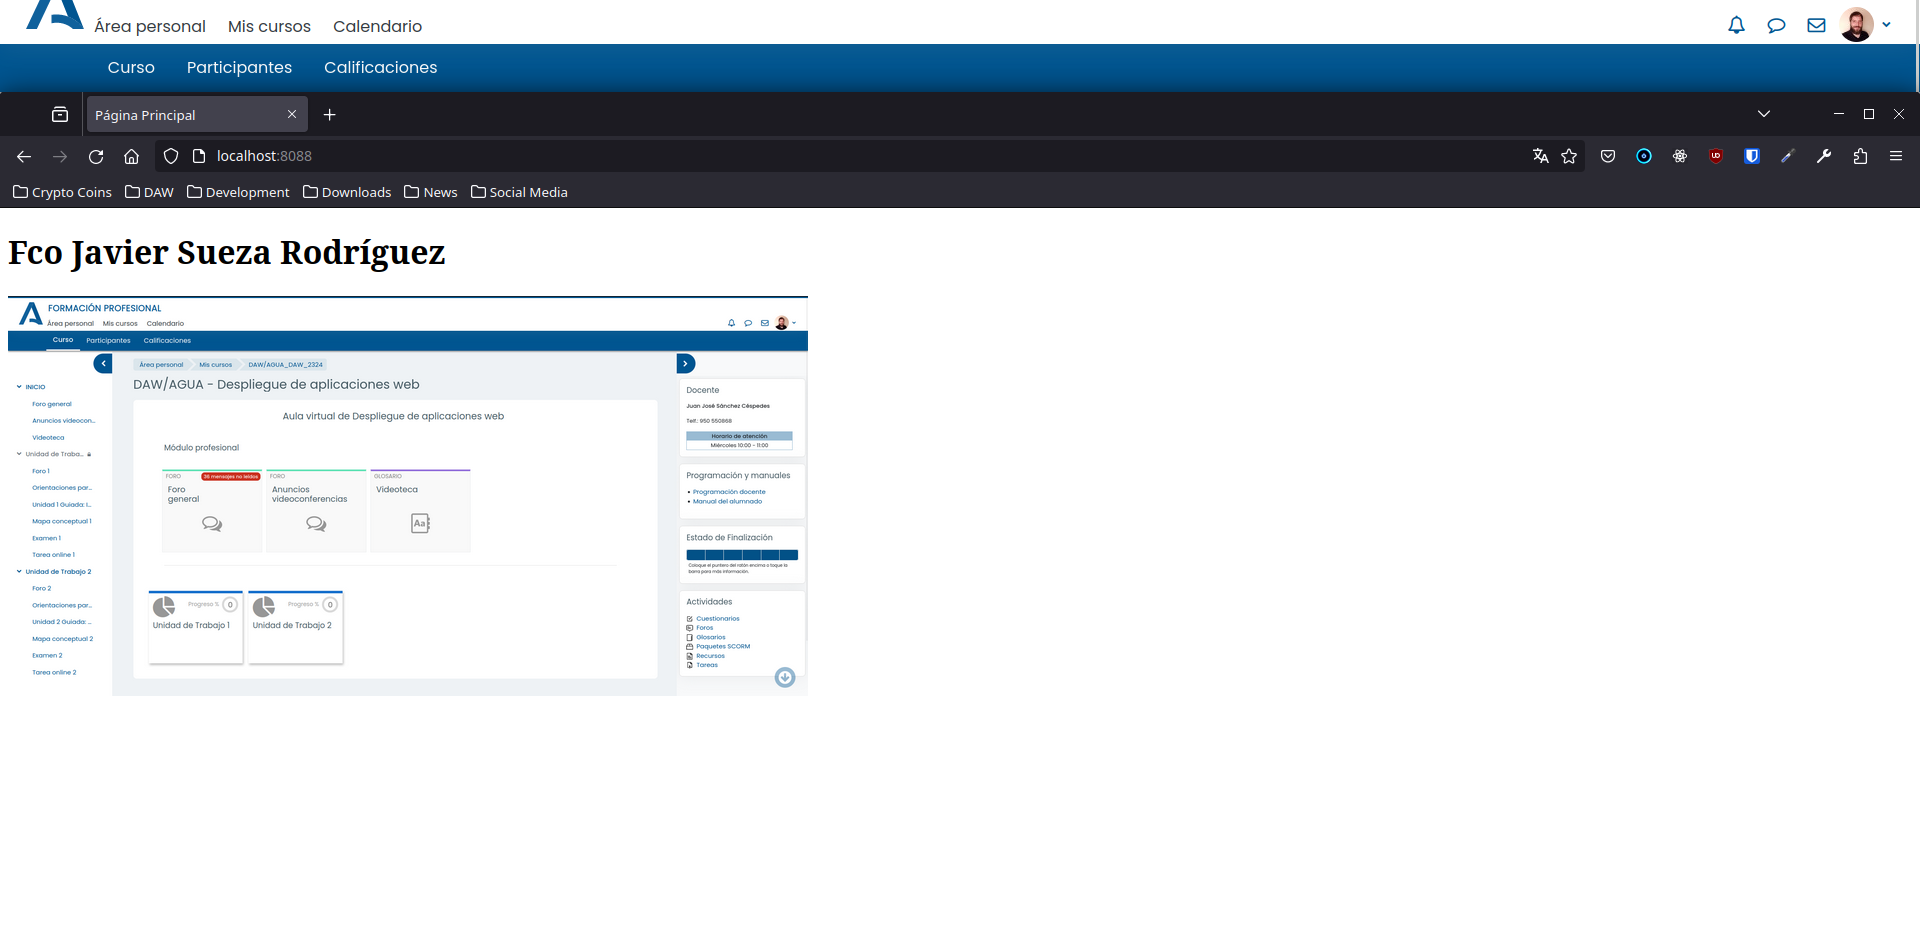
\includegraphics[scale=0.30]{apache-home-change.png}
      \end{figure}
\end{itemize}

\section{Ejercicio 4: Haciendo las Comunicaciones Más Seguras}
\subsection{Enunciado}
Partiendo de la instalación de Apache del ejercicio anterior, instala un certificado de seguridad (SSL) en tu servidor y habilita el módulo de Apache correspondiente para que funcione correctamente. Comprueba desde tu navegador que ahora puedes acceder al servidor usando el protocolo seguro (https).

\subsection{Solución}
En este ejercicio vamos a instalar un certificado SSL en Apache, con lo siguientes pasos:

\begin{enumerate}
    \item En primer lugar, se ha generado el certificado con \textbf{openssl}, que ya estaba instalado, y se ha almacenado en el directorio \textbf{\textit{/etc/apache2/personal-ssl}}, que se ha creado mediante \textbf{mkdir}. A continuación se ha usado el comando \textbf{\textit{make-ssl-cert}} para generar el certificado, mostrando el menú que podemos ver en la siguiente captura.

    \begin{figure}[H]
        \centering
        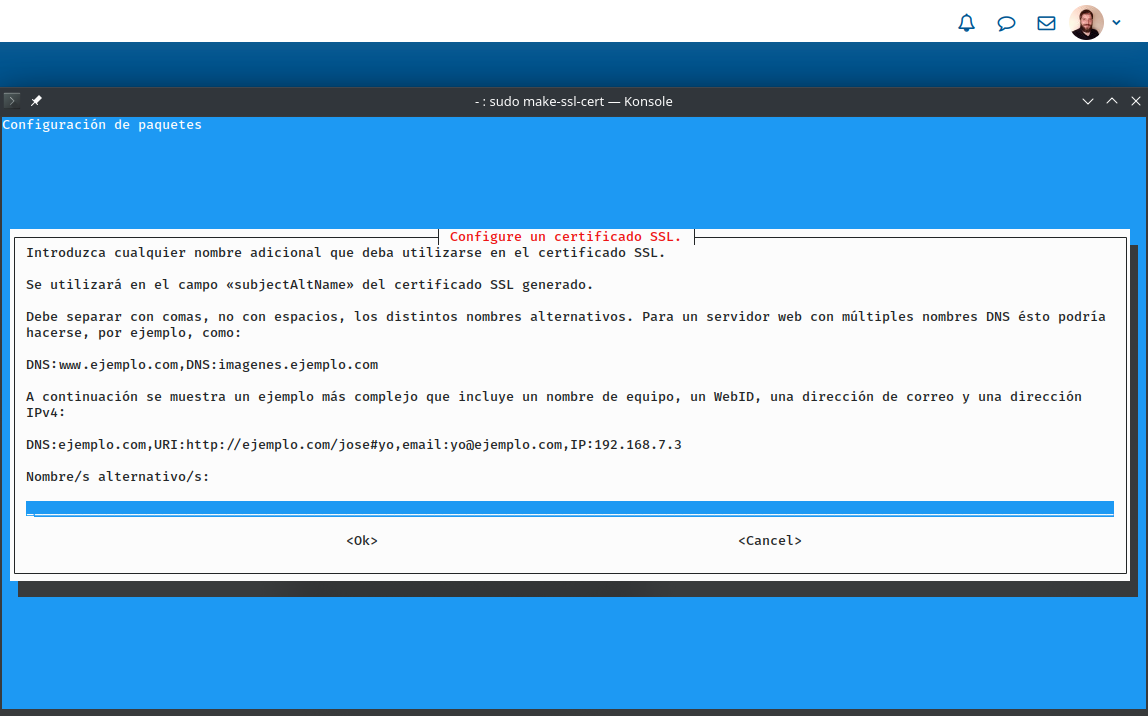
\includegraphics[scale=0.32]{ssl-creation.png}
    \end{figure}

    Tras completar los datos, se ha generado el archivo \textbf{\textit{apache.pem}} en la carpeta anteriormente mencionada.

    \item El siguiente paso es \textbf{cambiar la configuración} de Apache, para indicarle el nuevo directorio donde deberá buscar el certificado SSL. En la siguiente captura podemos ver la modificación que se ha realizado en el archivo \textbf{/etc/apache2/sites-available/default-ssl.conf}.

    \begin{figure}[H]
        \centering
        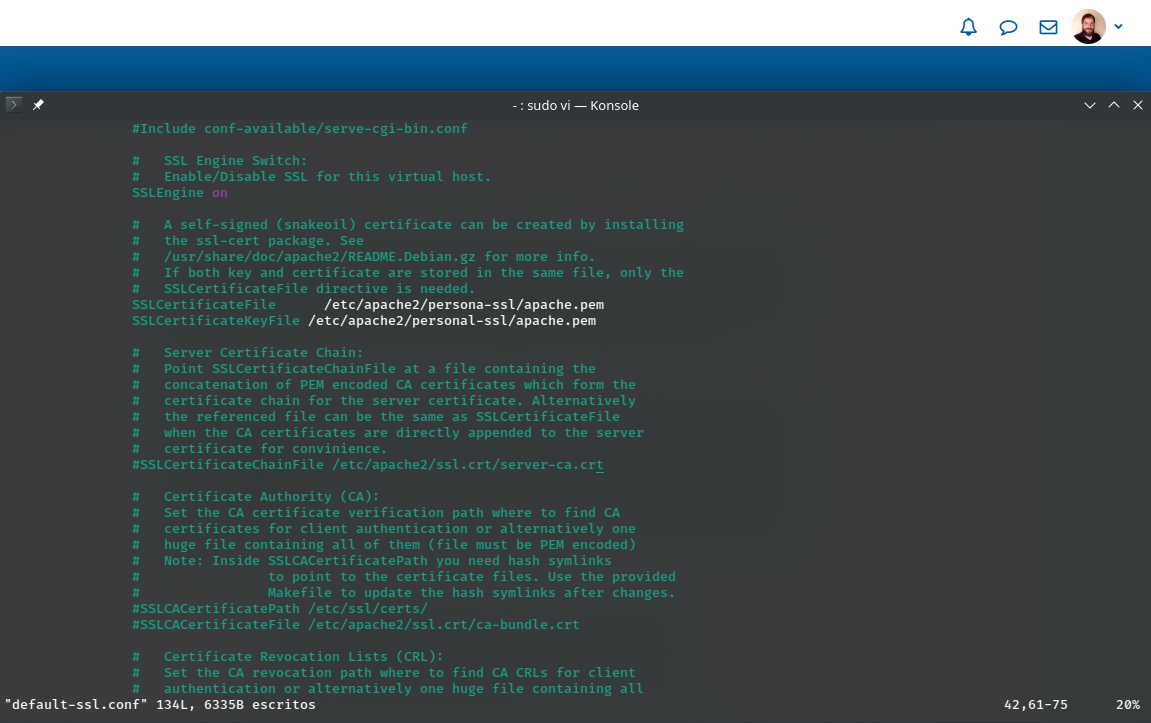
\includegraphics[scale=0.32]{ssl-apache.png}
    \end{figure}

    \item Tras comprobar que está habilitado el puerto 433 cuando el módulo SSL está cargado, se ha \textbf{cargado el módulo} ssl en Apache y se ha \textbf{añadido a avaible-sites} el fichero default-ssl, para posteriormente resetear el servidor web. En la siguiente captura, vemos la secuencia de comandos empleada.

        \begin{figure}[H]
        \centering
        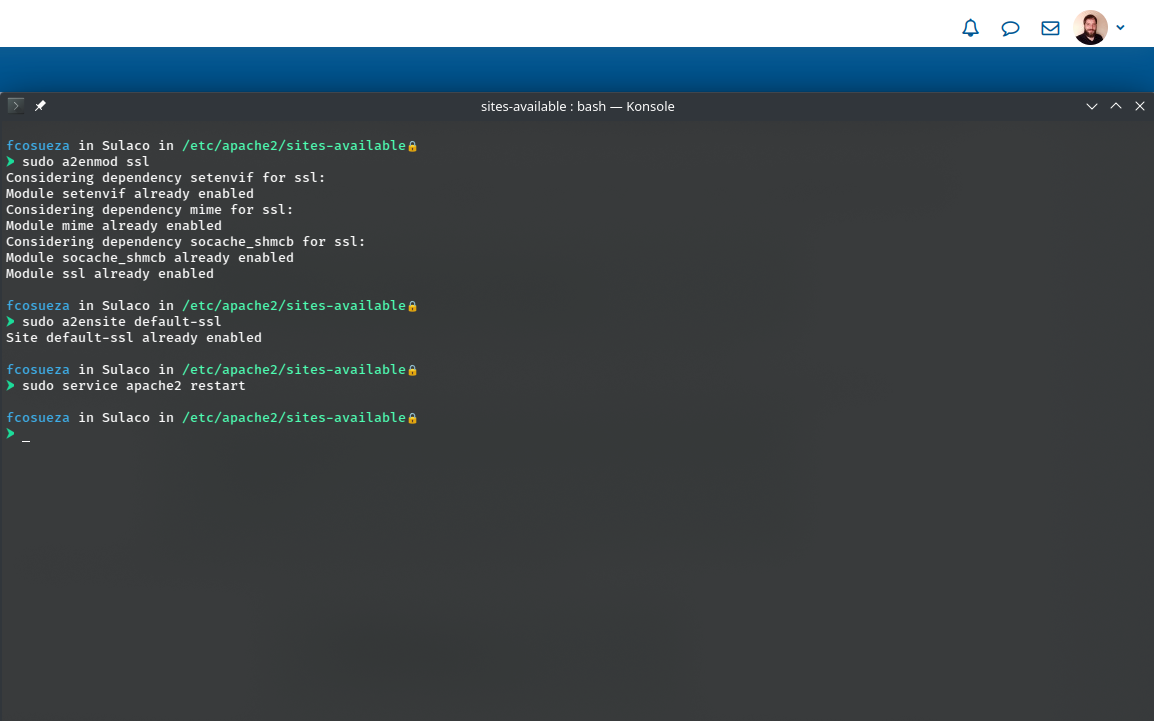
\includegraphics[scale=0.40]{ssl-apache-mod.png}
    \end{figure}

    \item Por último se ha comprobado que funciona correctamente la conexión SSL en servidor. Para ello, nos hemos conectado al \textbf{localhost} usando la dirección \textbf{https://localhost}. No hemos empleado otra dirección porque cuando se configuró el certificado no se especificaron nombres alternativos, para poder conectarnos de esta forma sin necesidad de modificar más ficheros. En la siguiente captura se ve como nos conectamos mediante SSL al servidor.

    \begin{figure}[H]
        \centering
        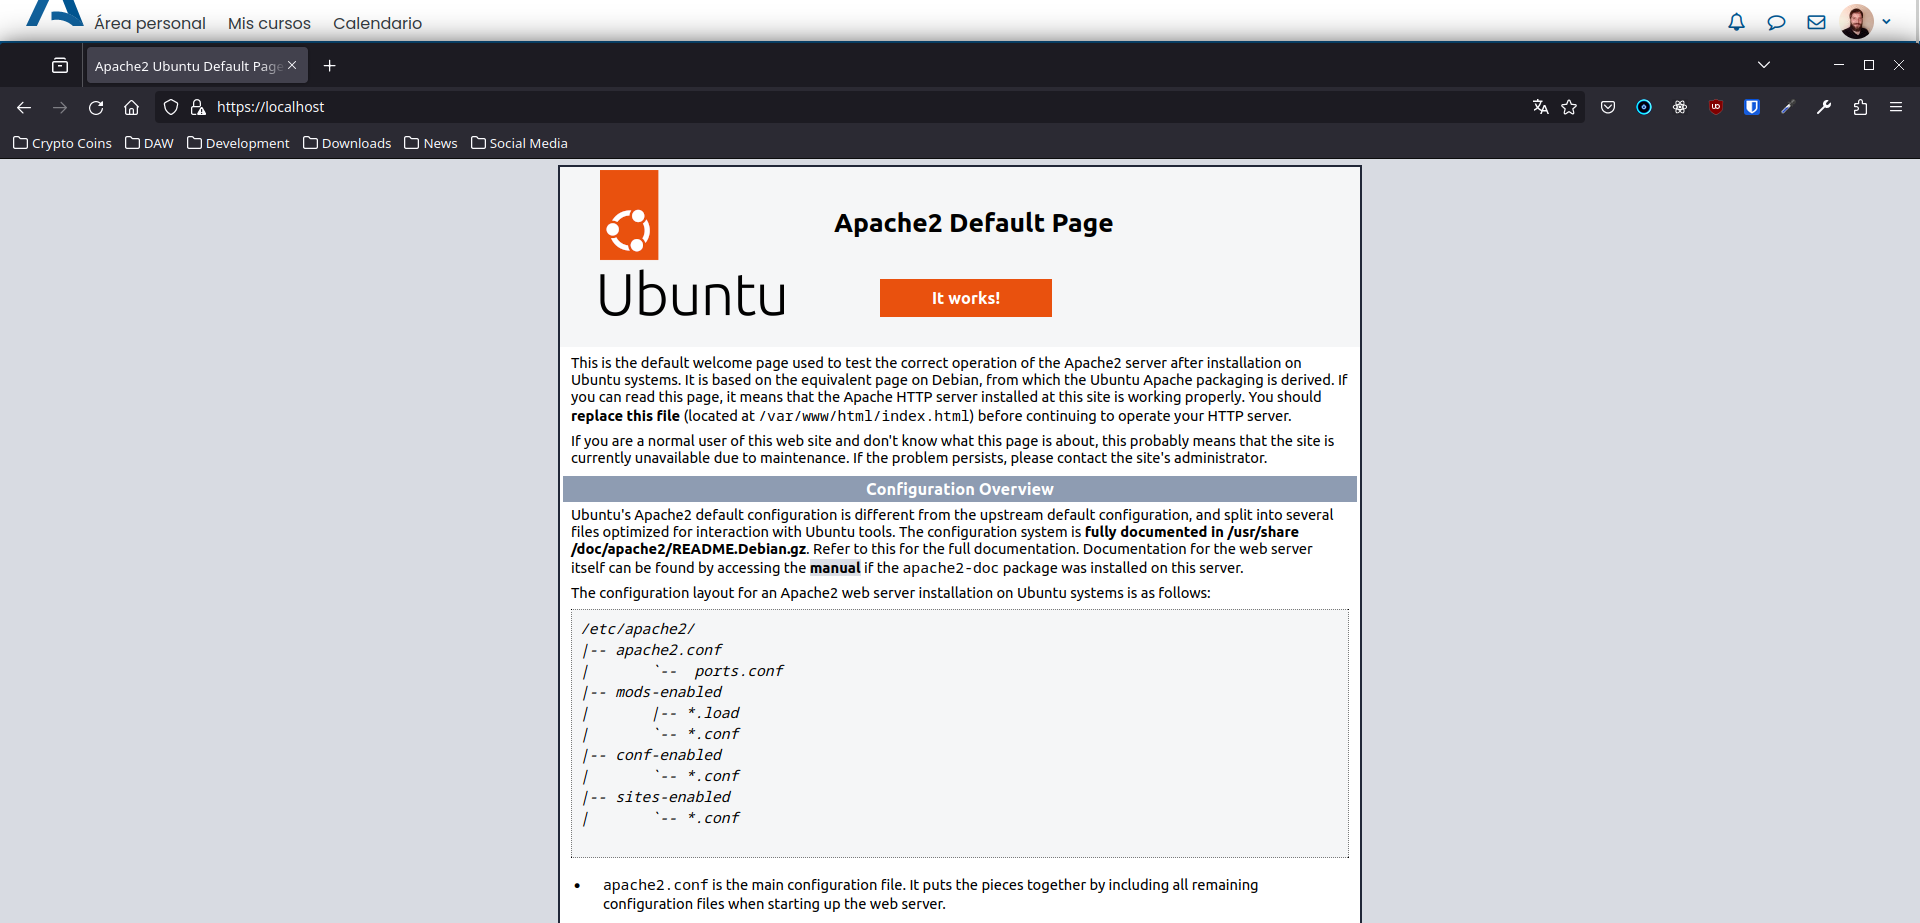
\includegraphics[scale=0.30]{ssl-check.png}
    \end{figure}

    \textbf{NOTA:} La página que se muestra es la que viene por defecto con Apache, ya que después del ejercicio anterior se han revertido los cambios en esta página para que vuelva a mostrar la que viene por defecto.
\end{enumerate}

\section{Ejercicio 5: Instalador de un Servidor de Aplicaciones}
\subsection{Enunciado}
Partiendo de la instalación de Apache del ejercicio 3, realiza la instalación del servidor de aplicaciones \textbf{Apache Tomcat} (es recomendable instalar una versión lo más reciente posible, tomcat10). \textbf{Importante:} para esta actividad solo hay que hacer la instalación y comprobar desde nuestro navegador que tenemos acceso a la página principal del servidor de aplicaciones. No hay que configurar el acceso al panel de administración ni crear usuarios.

\subsection{Solución}
En este ejercicio vamos a realizar una instalación básica del servidor de aplicaciones Tomcat, probando a continuación que se ha instalado correctamente desde un navegador. Los pasos que se han seguido han sido los siguientes:

\begin{enumerate}
    \item En primer lugar, hemos descargado la distribución binaria de Tomcat mediante el comando \textbf{\textit{wget}}. En nuestro caso, se ha descargado la \textbf{versión 10.1.6}, como podemos ver en la siguiente captura.

    \begin{figure}[H]
        \centering
        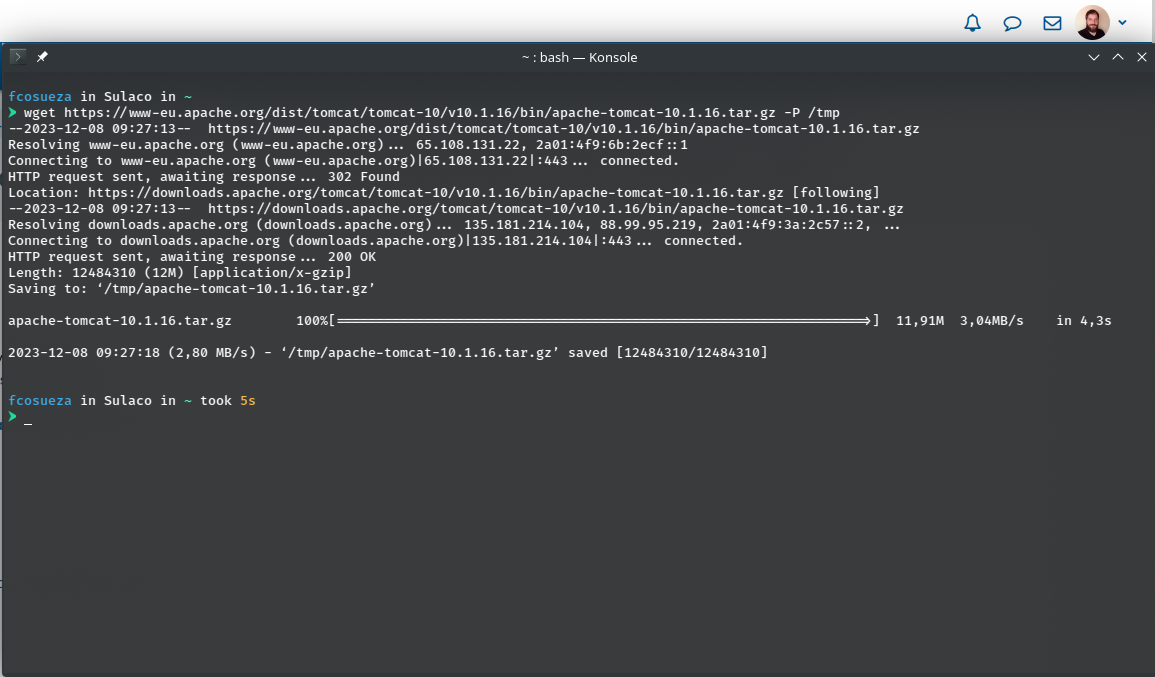
\includegraphics[scale=0.40]{tomcat.png}
    \end{figure}

    \item El siguiente paso ha sido descomprimir el archivo descargado en la carpeta \textbf{\textit{/opt}}, que va a ser donde se almacene definitivamente la distribución binaria de Tomcat. Para ello hemos usado el comando \textbf{\textit{sudo tar -zxvf /tmp/apache-tomcat-10.1.16.tar.gz -C /opt/}}.

    \item Como vamos a realizar una instalación básica sin mucha configuración, ya solo nos queda ejecutar el script de inicio de Tomcat. En este caso, hemos ejecutado el script \textbf{startup.sh}, que se encuentra en al carpeta \textbf{\textit{bin/bin}} del directorio de Tomcat.

    \item Por último, nos hemos conectado al \textbf{localhost} usando el puerto \textbf{8080} para comprobar que se esta ejecutando Tomcat correctamente, y como podemos ver en la siguiente captura, su ejecución e instalación se ha realizado correctamente.

    \begin{figure}[H]
        \centering
        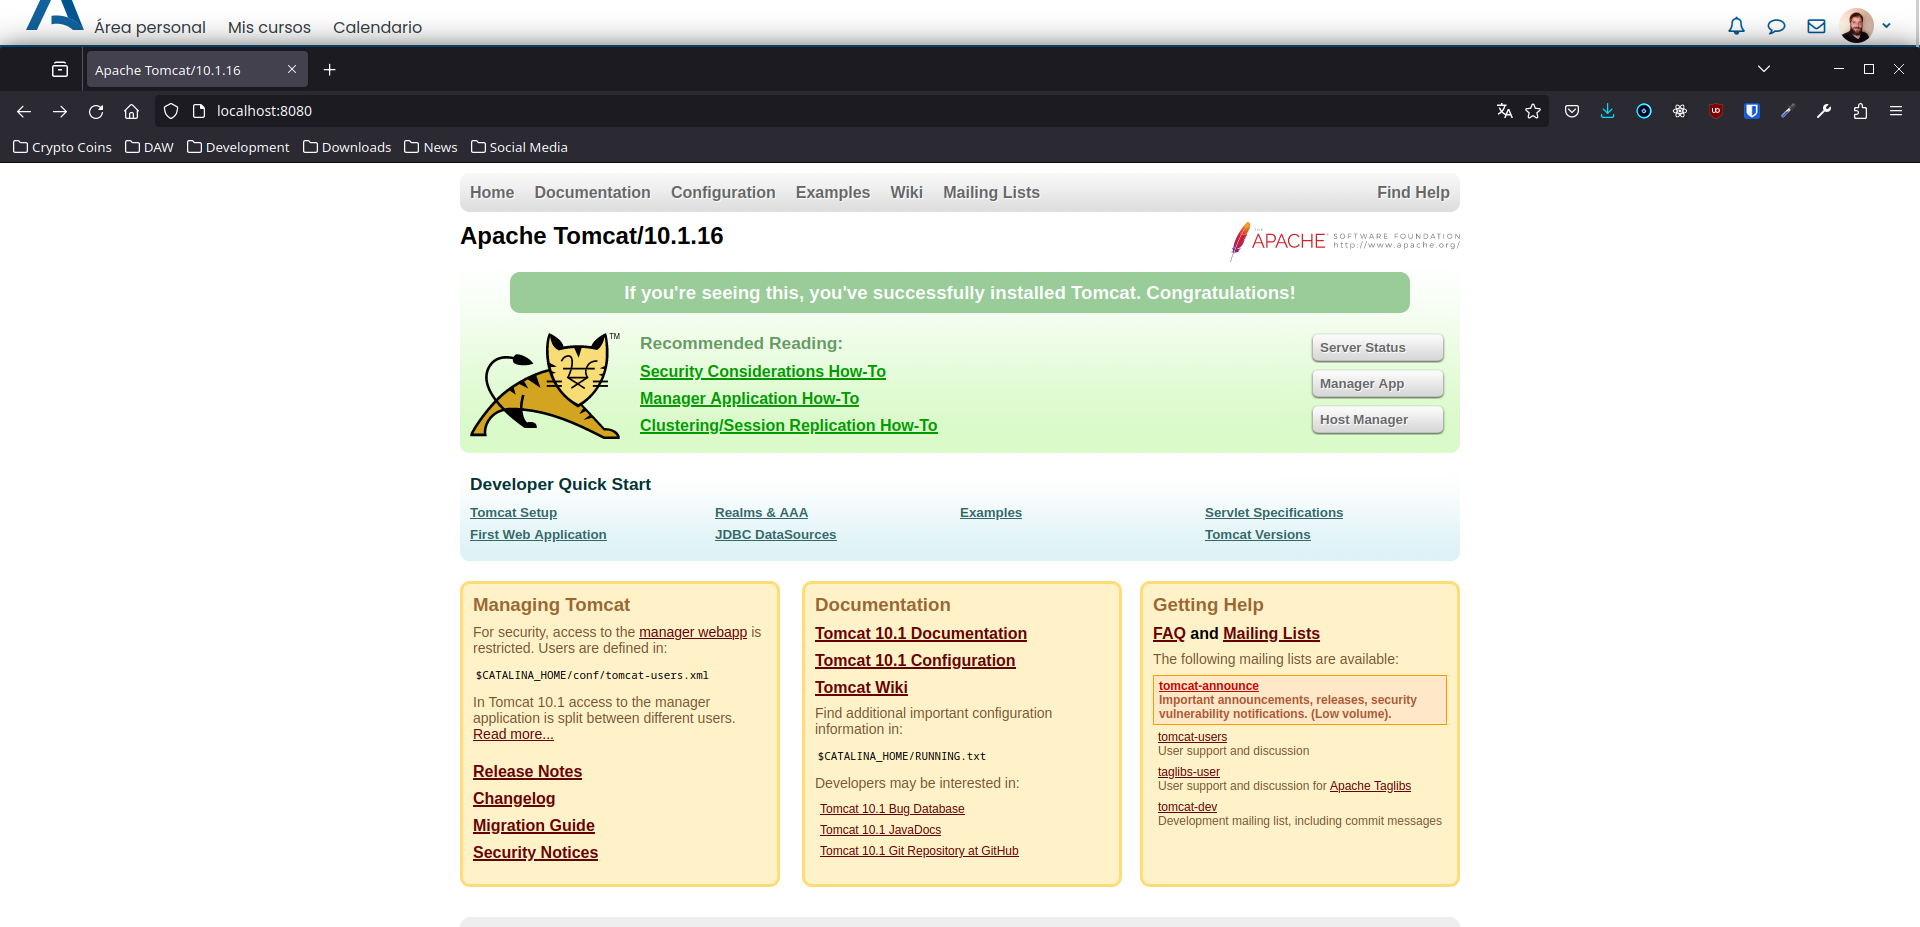
\includegraphics[scale=0.30]{tomcat-installed.png}
    \end{figure}
\end{enumerate}

\section{Ejercicio 6: Hosts Virtuales}
\subsection{Enunciado}
Ya sabemos que Apache permite tener más de un sitio web en un servidor, donde cada sitio puede estar asociado a un dominio diferente. Revisa el punto 5 de la documentación y explica qué es, para que se utiliza y cuál es la diferencia entre virtualhost por nombre y por IP. Pon un ejemplo de configuración de cada uno, usando las directiva 'VirtualHost', incluyendo capturas del fichero de configuración.

\subsection{Solución}
Los \textbf{VirtualHosts} son un mecanismo de Apache que nos permite que un servidor albergue diferentes webs con diferentes dominios, manteniendo cada dominio y su estructura de directorios independiente de los demás. Los Virtualhost se pueden utilizar de varias formas diferentes, aunque las más comunes son:

\begin{itemize}
    \item \textbf{VirtualHost por Nombre}: en este tipo de VirtualHosts tenemos varios dominios asociados a una misma IP. Cuando un cliente se conecta a dicha IP, se servirá una página u otra dependiendo del dominio que se especifica.

    \item \textbf{VirtualHost por IP}: en este caso, hay diferentes IPs asociadas a la misma máquina y estas se asocian con las diferentes páginas que alberga el servidor, por lo que se servirá una página u otra dependiendo de la dirección IP que especifique el cliente.
\end{itemize}


Para configurar los Virtualhost en Ubuntu, que es el sistema que estamos empleando se deben añadir un archivo a la carpeta \textbf{/etc/apache2/sites-avaibles/}, donde se especifiquen las diferentes directivas del servidor. Habrá que añadir un archivo por cada Virtualhost que queramos, y una vez que que estén bien definidos, deberemos copiarlos o crear un enlace simbólico en la carpeta \textbf{/etc/apache/sites-enabled}. A continuación, vamos a mostrar dos ejemplos de configuración de VirtualHosts.

El primer ejemplo es un \textbf{VirtualHost por nombre} que ya teníamos configurado para la asignatura DWES. En este caso, en este caso, además de las opciones habituales, se ha añadido una directiva para que no se puede acceder a la \textbf{carpeta nbproject} desde el servidor, ya que es irrelevante para el sitio web ya que contiene la información del proyecto de Netbeans.

\begin{figure}[H]
    \centering
    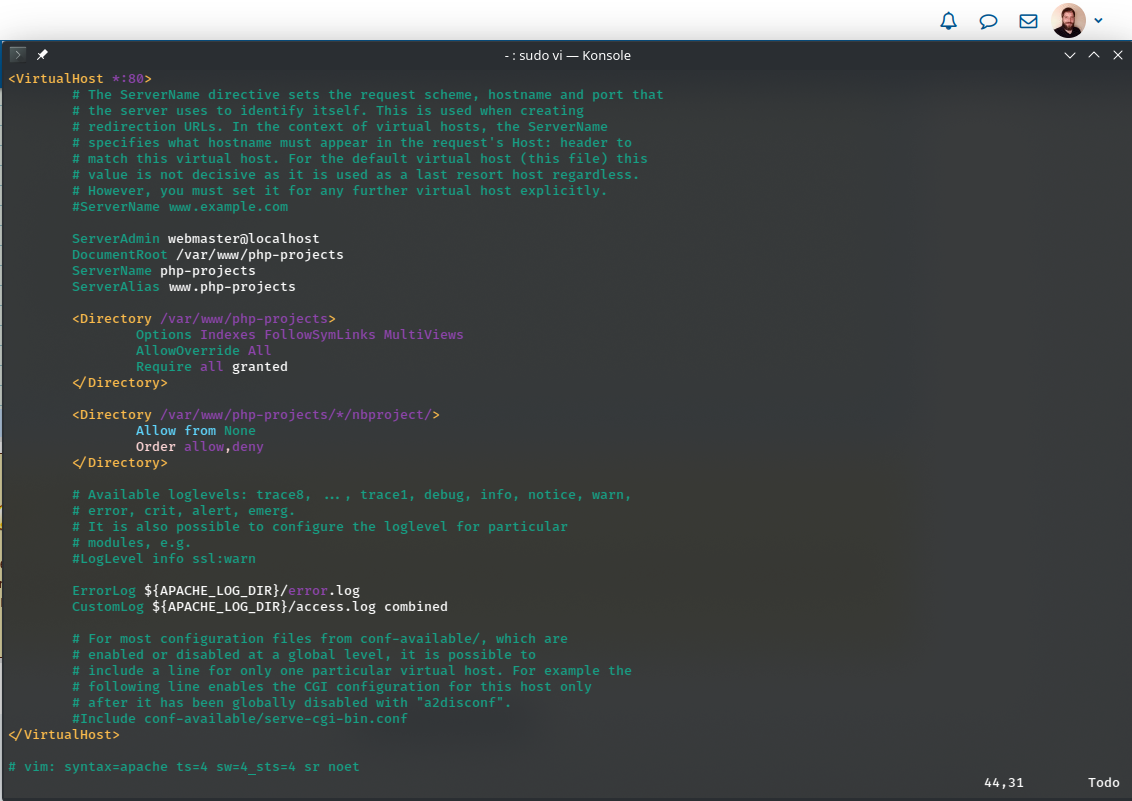
\includegraphics[scale=0.40]{virtual-name.png}
\end{figure}

Ahora vamos a mostrar un ejemplo del fichero de configuración de un \textbf{Virtualhost por IP}. En este caso como no teníamos ninguno configurado, se ha creado desde cero y hemos simulado dos hosts virtuales a las paginas de las asignaturas de programación y desarrollo web en el entorno cliente. El fichero, quedaría como podemos ver a continuación.

\begin{figure}[H]
    \centering
    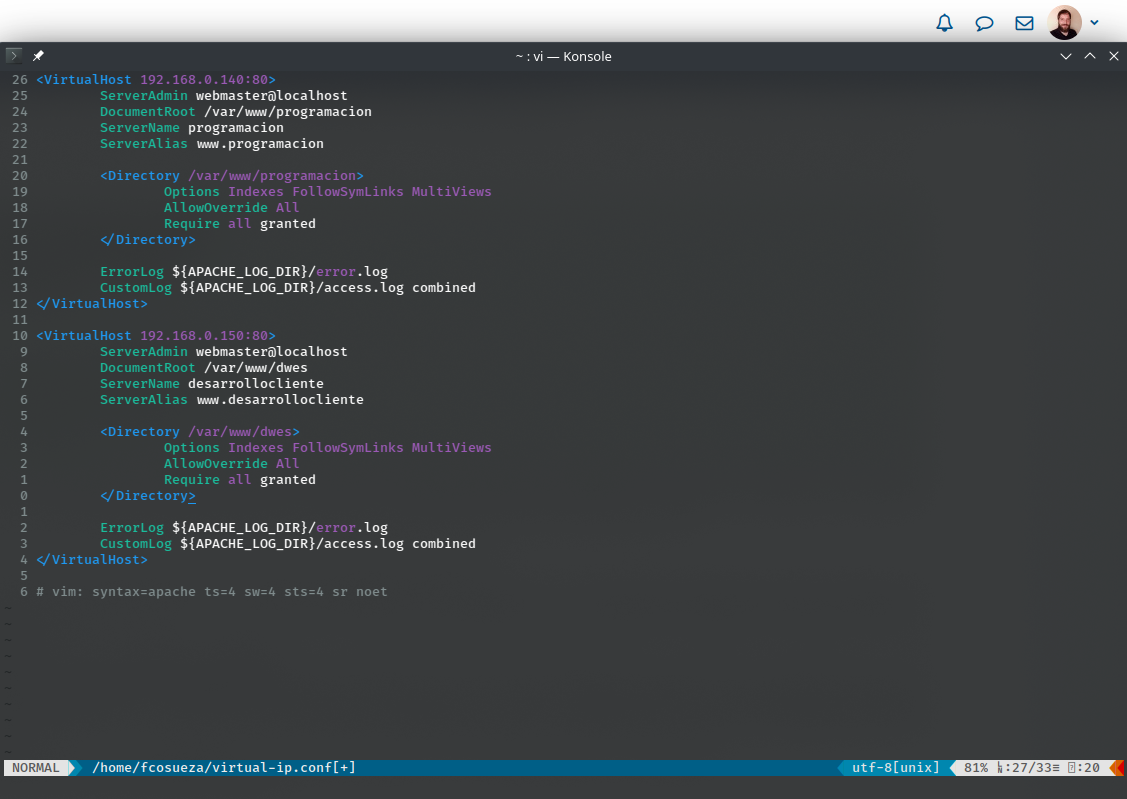
\includegraphics[scale=0.40]{virtual-ip.png}
\end{figure}






% Bibliography

%\newpage
%\bibliography{citas}
%\bibliographystyle{unsrt}

\end{document}